\chapter{Design}%
\label{cha:design}

%In this chapter, you should present your solution in detail but at a conceptual level. This means that you explain the overall design including your motivation for this design but you do not provide details on the actual implementation of your design (e.g., in which programming language you wrote it, how the software is structured and so on). This means that you should also point out the aspects where you had different design options and in which points they differ. A good approach to write this chapter is to make yourself aware of the different aspects and design problems that need to be addressed in your design. To do so, you can then proceed repeatedly in three steps:
%\begin{enumerate}
 %  \item Explain a design problem that needs to addressed by the solution (e.g. to enable anonymous communication over the internet, participants need to be able to send messages to each other without revealing identifying to the corresponding receiver).
  % \item Discussion of design choices (e.g. Mix Networks, DC-Networks, etc.) with regards to the requirements from the previous chapter and identification of the most promising choices.
%\end{enumerate}
%After the second step, you start the next iteration by identifying design problems that arise when you want to use the most promising design choice. For example, if Mix networks turn out to be the most promising approach for your requirements, you then need to address the question how the mix network should be designed (e.g. how are mix nodes chosen by the users of the anonymization network? How do mix nodes process messages?). Once you identified the most promising solutions to that, you can then start the next iteration and so on until there are no more open design questions that you are aware of.
Zuerst erläutere ich die meiner Meinung nach bestehende Notwendigkeit für eine Taxonomie. Dann definiere ich die Kontextkategorien meiner Taxonomie. Danach definiere ich in welcher Form die Kontextinformationen in den einzelnen Kategorien vorliegen müssen und wie man Informationen aus unterschiedlichen Quellen in einer für IDS-Signaturen verwendbaren Form gewinnt. Zusätzlich gehe ich noch darauf ein welchen Anforderungen ich an ein IDS stelle und welche Schwächen ich in dem von mir gewählten IDS mithilfe von Kontextsensitivität lösen will. Abschließend bewerte ich wie gut sich die benötigten Kontextinformationen gewinnen lassen. 

\section{Notwendigkeit einer Taxonomie}
%TODO “Based on the evaluation of context categorisation, it is evident that no single categorisation scheme can accommodate all the demands” ([Perera et al., 2014, p. 423]
Die Evaluation verschiedener Kategorisierungsschemata zeigt das keine Kategorisierung allen Ansprüchen gerecht werden kann\cite{perera_context_2014}.
\section{ Erstellung einer Kontexttaxonomie }
Im folgenden möchte ich meinen Versuch einer Kombination der bereits vorgeschlagenen Kategorisierungsschemata erläutern. Dazu lege ich zuerst die Definition der einzelnen Kategorien im Bezug auf kontextsensitive Zugriffskontrolle fest. Die Kategorien müssen dafür, abhängig davon mit welchem Fokus sie der jeweilige Autor konstruiert hat, mehr oder weniger stark angepasst werden.
\subsection{Konzeptionell}
Einordnung anhand der Bedeutung des Kontextes und der begrifflichen Beziehungen.
\subsubsection{Primär}
%“Any information retrieved without using existing context and without performing any kind of sensor data fusion operations (e.g. GPS sensor readings as location information).” 
Kontextinformationen die gesammelt werden können ohne bereits vorhandene Daten zu verwenden oder zu kombinieren. \cite{abowd_towards_1999}
\subsubsection{Sekundär}
%"Any information that can be computed using primary context. The secondary context can be computed by using sensor data fusion operations or data retrieval operations such as web service calls (e.g. identify the distance between two sensors by applying sensor data fusion operations on two raw GPS sensor values). Further, retrieved context such as phone numbers, addresses, email addresses, birthdays, list of friends from a contact information provider based on a personal identity as the primary context can also be identified as secondary context.” 
Kontext der durch das verarbeiten von primärem Kontext erschlossen werden kann. Dies kann durch die Kombination einzelner Datenpunkte einer oder mehrerer Kategorien oder durch Abfragen weiterer Informationen mithilfe der primären Informationen geschehen \cite{abowd_towards_1999}.
\subsection{Betrieblich}
Wie schon in der Analyse bereits vorgeschlagener Kategorien bedeutet die betriebliche Kategorisierung: "Einordnung anhand dessen wie der Kontext akquiriert, modelliert und behandelt wird".
\subsubsection{Zeit}
Zu welcher Zeit ein Zugriffsanfrage erfolgt.
\subsubsection{Ort}
Von welchem Ort eine Zugriffsanfrage stammt.
\subsubsection{Identität}
Wer Zugriff auf eine Ressource erfragt.
\subsubsection{Aktivität}
Was in einer Situation passiert bzw. welche Aktion eine Entität ausführt.
\subsubsection{Grund}
%--------------------------
\subsection{Historie}
Die Historie einer Entität ist in meiner Taxonomie zweigeteilt. Sie besteht aus:
\begin{enumerate}
\item{Einem aktiven Teil also ihrem Verhalten, beispielsweise früheren Verbindungen bzw. Verbindungsanfragen}
\item{Einem passiven Teil also dem Zustand der für sie charakteristischen Attribute, beispielsweise einem Nutzernamen oder die Versionsnummer eines bestimmten Programms}
\end{enumerate}
Die Existenz einer Historie trifft die implizite Annahme das eine Entität eindeutig und über einen längeren Zeitraum im Netzwerkverkehr identifizierbar ist.
\subsubsection{Dynamik}
Wie 
 %TODO im Kapitel Hintergrund%
 beschrieben können sich die Werte, aus denen sich die Historie einer Entität zusammensetzt, je nach dem welchem Teil sie zugeordnet werden, verschieden oft ändern.
Statische Messgrößen ändern dabei ihre Werte nie oder nur sehr selten. Dynamische Messgrößen hingegen sehr oft. In meinem Fall erachte ich dabei eine Kategorisierung in jährlich, monatlich, wöchentlich, täglich, stündlich, minütlich und sekündlich für sinnvoll.
\subsubsection{Raten}
Die Historie ist weiterhin in 3 verschiedene Bereiche unterteilt. Abängig davon wo die Änderung auftritt und ob das IDS oder eine Entität die Aktualisierung des Wertes auslöst.
\subsubsection{Änderungsrate} 
Gibt an wie oft eine Entität eine Werteänderungen mitteilt.
\subsubsection{Abtastrate}
Wie oft Werte einer Entität vom IDS abgefragt bzw aktualisiert werden.
\subsubsection{Abfragerate}
Wie oft Werte im Netzwerk von einer Entität, die nicht das IDS ist, abgefragt werden.
%--------------------------
\subsection{Protokoll}
Kategorisierung anhand des verwendeten Kommunikationsprotokolls. Orientiert sich am ISO/OSI-Referenzmodell \cite{day1983osi}.
\subsubsection{Anwendung}

\subsubsection{Transport}
\subsubsection{Netzwerk}

\subsection{Logisch}
\subsubsection{Attribute der Entitäten}
Kategorisierung von Kontextinformationen abhängig davon welche Art von Entität sie betreffen.
Diese Unterscheidung setzt genauso wie die Historie eindeutig identifizierbare Entitäten voraus.
\paragraph{Gerät}
Informationen die sich auf ein spezifisches Gerät beziehen
\begin{enumerate}
\item{Ein Gerät ist beispielsweise einen Router oder das Endgerät eines Nutzers. }
\item{Informationen können beispielsweise die Liste an installierter Software, die Menge laufender Prozesse oder die Auslastung der Hardwarekomponenten sein.}
\end{enumerate}
\paragraph{Nutzer}
Informationen die sich auf einen Nutzer beziehen.
\begin{enumerate}
\item{Ein Nutzer im Sinne eines Computersystems und keine physische Person. So kann eine physische Person durchaus mehrere verschiedene logische Nutzerkonten haben. }
\item{Informationen können die Zugriffsrechte oder %TODO
umfassen.}
\end{enumerate}
\paragraph{Anwendung}
Informationen die sich auf eine Anwendung beziehen.
\begin{enumerate}
\item{}
\end{enumerate}
\subsection{Verhaltensbezogen}
Einordnung der Kontextinformationen abhängig davon sie der für den Anwendungsfall definierten Normen entsprechen.
\subsubsection{Erwartetes Verhalten}
Informationen die dem
\subsubsection{ungewöhnliches Verhalten}
\newpage
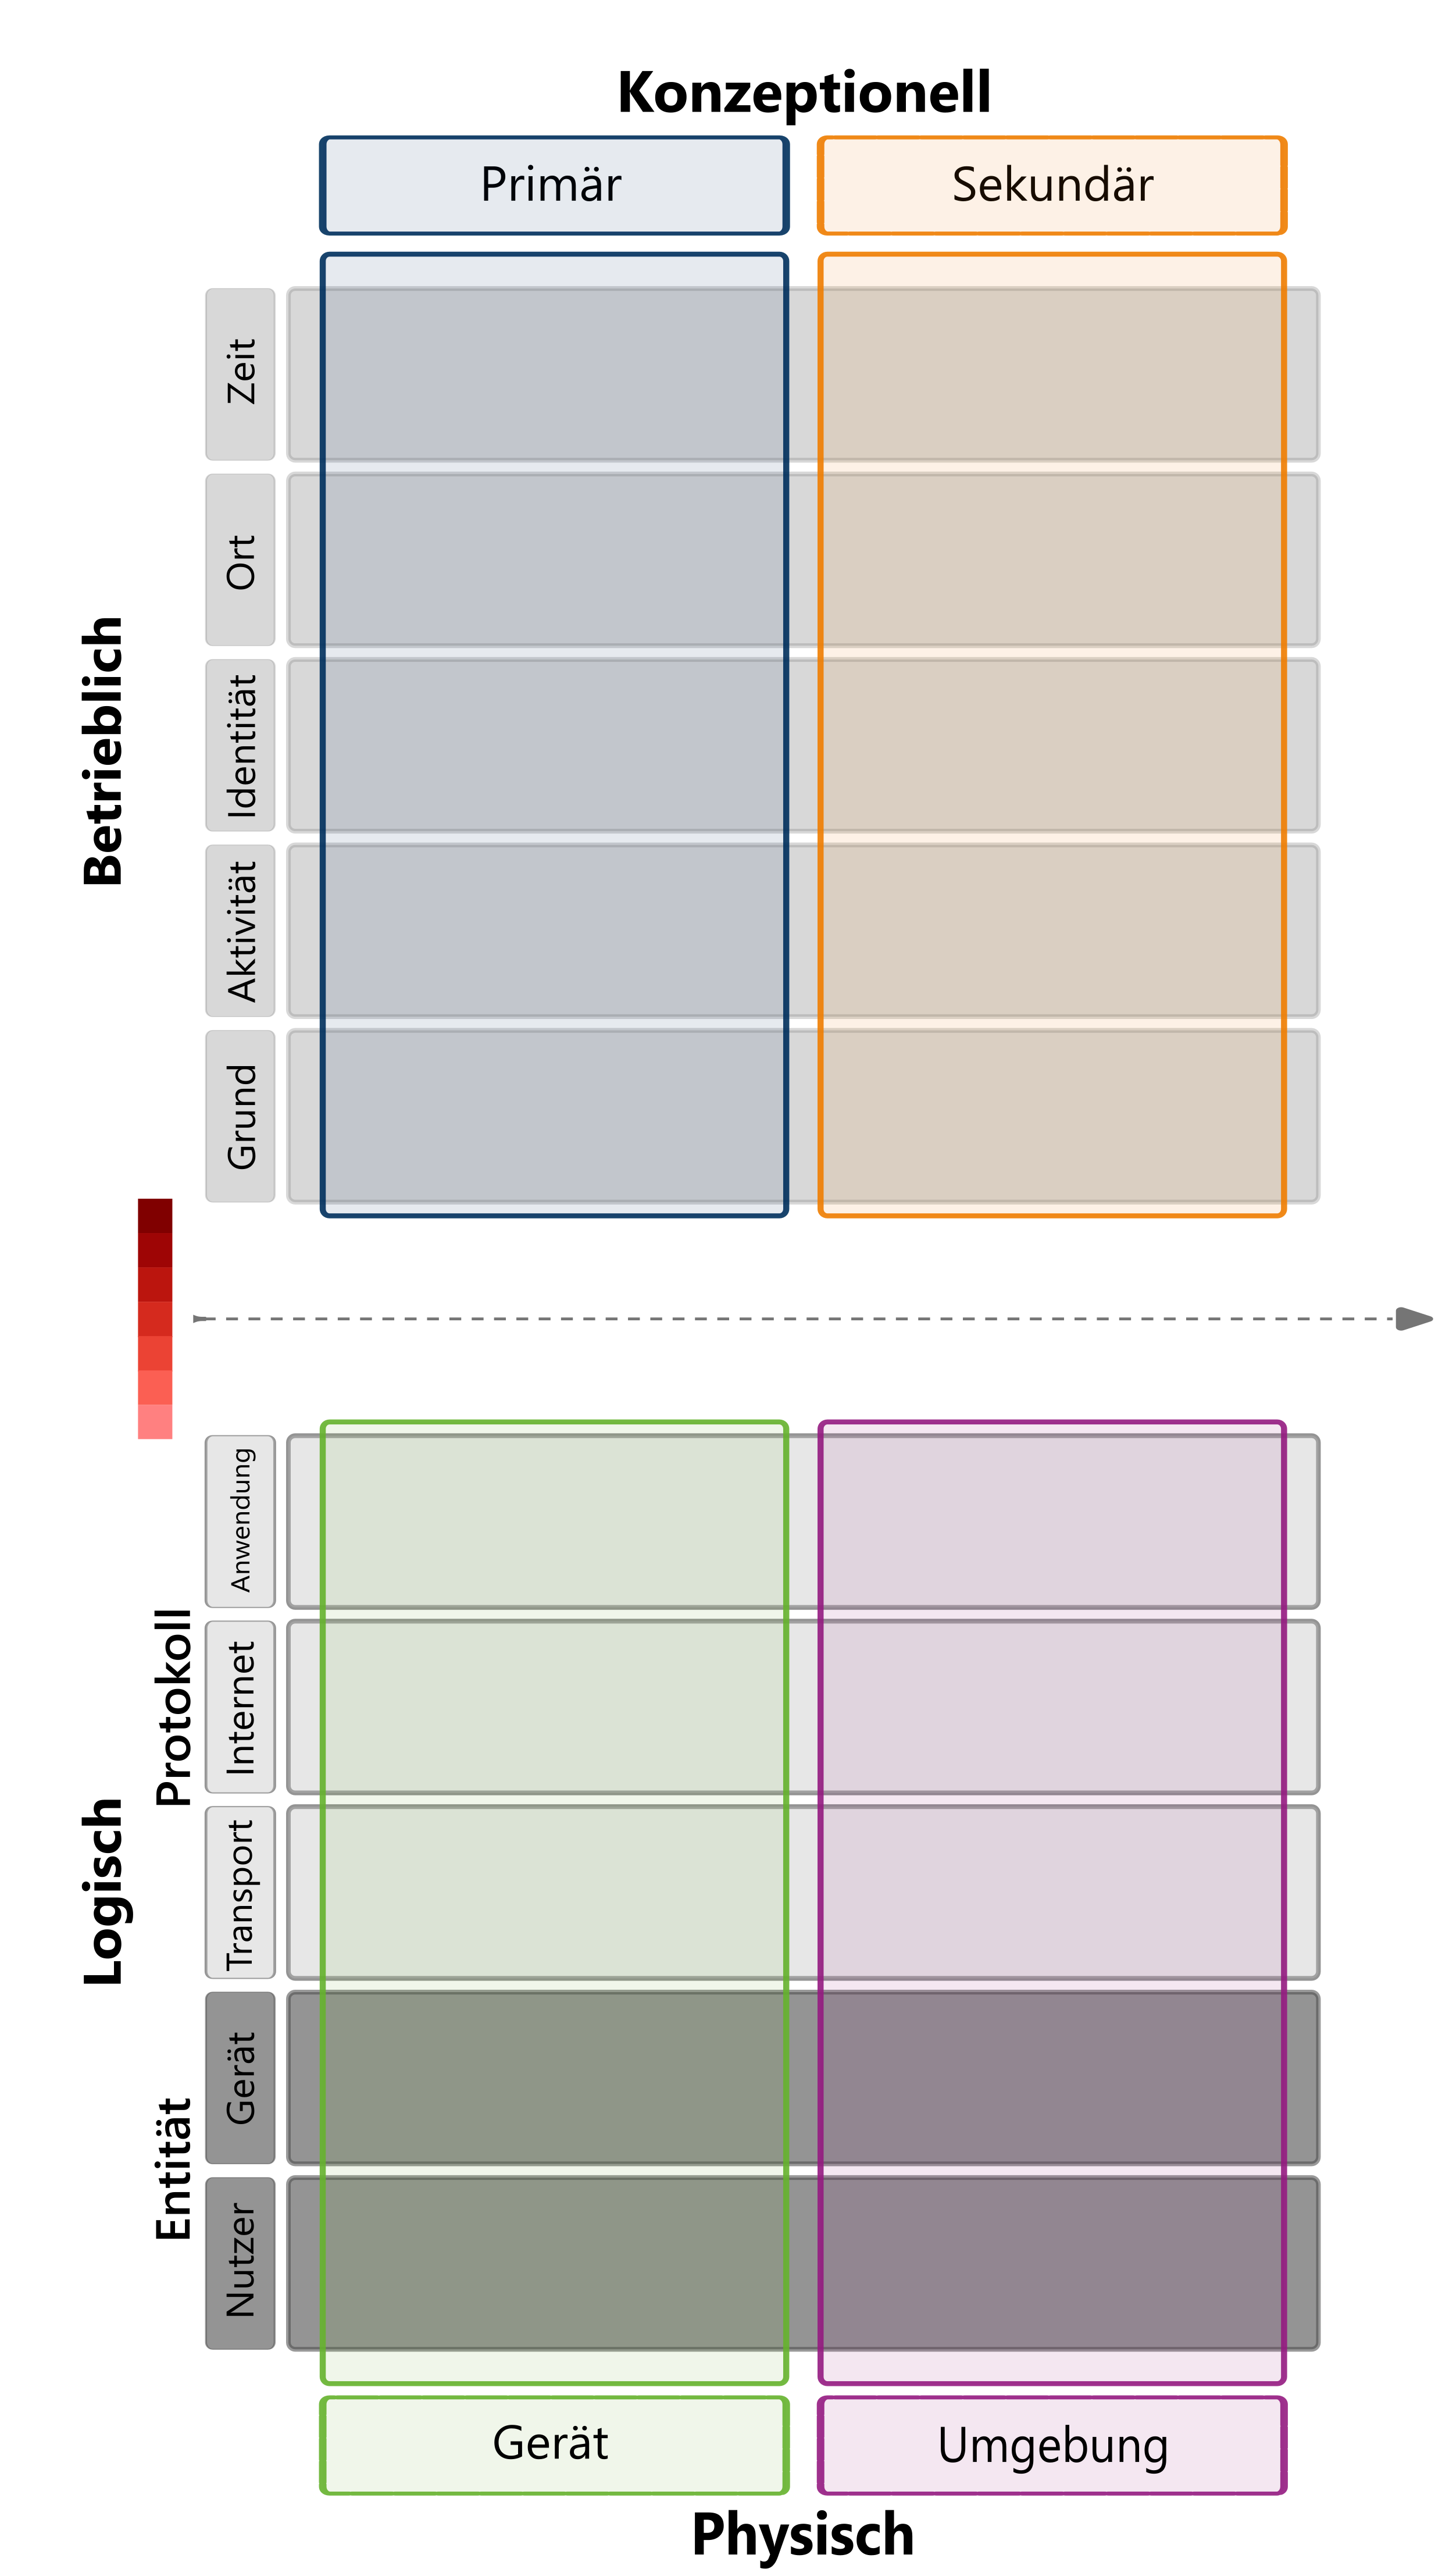
\includegraphics[width=13cm,height=24.1cm]{test}
\section{Werte einer Kategorie}
%TODO work in Progress

\subsection{Historie}
%Scr-IP/Port + Dest-IP/Port
%Zeitpunkt
%Protokoll
%Paketlänge
%Verbindung möglich
%Verbindung zugelassen
\section{Kontextgewinnung}
%Wo genau bekommt man Kontextinformationen her 
%TODO  A Context Aware Network-IDS
- network (open ports) | Nessus
- devices in network | Configuration Management Database (CMDB), nmap   
- cve reference - yes/no
- protocol header

